\documentclass[11pt,a4paper]{article}
\usepackage{cmap}
\usepackage[utf8]{inputenc}
\usepackage[german]{babel}
\usepackage[left=1.5cm,right=1.5cm,top=1.5cm,bottom=1.5cm]{geometry}
\author{Andreas Hemmetter}
\let\footruleskip\undefined %undefine footruleskip
\usepackage{fancyhdr}
\usepackage{multicol}
\usepackage{microtype}
% \usepackage{textcomp}
% \usepackage{amsthm}
\usepackage{framed}
\usepackage{multirow}
\usepackage{xhfill}
\usepackage{makecell}
\usepackage{tabularx}
% \usepackage{bbold}
% \usepackage{amssymb}
\usepackage{hyperref}
\usepackage{booktabs}
\usepackage{graphicx}
\usepackage{setspace}
\usepackage{lettrine}
%\usepackage{braket}
% \usepackage{tikz}
% \usetikzlibrary{arrows}
\usepackage[sorting=none]{biblatex}
\addbibresource{refs-de.bib}
\AtBeginBibliography{\small} 
\definecolor{shadecolor}{rgb}{0.95, 0.95, 0.95}

\setlength{\headheight}{15.2pt}
\begin{document}
\pagestyle{fancyplain}
\fancyhf{}
\rhead{\textbf{\textit{Weltföderation}} - \href{mailto:ahemmetter@gmail.com}{A. Hemmetter} }
\rfoot{\scriptsize{ \href{https://creativecommons.org/licenses/by-sa/4.0/}{Creative Commons Namensnennung - Weitergabe unter gleichen Bedingungen 4.0 International Lizenz}}}
\begin{center}

\begin{tabular}[t]{@{}l}
\rule[4pt]{0.29\linewidth}{4pt}
\end{tabular}
\begin{tabular}[t]{@{}}
\fontsize{24pt}{10pt}
\textbf{Weltföderation}
\end{tabular}
\begin{tabular}[t]{r@{}}
\rule[4pt]{0.29\linewidth}{4pt}
\end{tabular}
\end{center}

\begin{multicols}{2}
\lettrine[lraise=0.1, lines=2]{\textsc{M}}{enschen} arbeiten seit über 12 000 Jahren an unserer Zivilisation. Durch Wissenschaft, Kunst, Philosophie, Technologie und harter Arbeit haben wir uns in eine gänzlich neue Welt katapultiert. Doch unsere politischen Einrichtungen haben bisher nicht aufgeholt: wir sind immer noch in den Strukturen der letzten Jahrhunderte gefangen.

\noindent Die Welt ist heute ein globales Dorf. Reisen, das Internet, Märkte und die Natur weben ein immer engeres Netz um uns Menschen. In dieser zusammenhängenden Welt sind Nationen zu klein geworden, als dass sie zur Lösung unserer wichtigsten Probleme etwas beitragen könnten. Eine demokratisch gewählte Regierung einer Weltföderation ist der beste Versuch, um uns selbst zu retten und das Potential der Menschheit freizusetzen.


\begin{shaded*}
\noindent \textit{Bis die Fahnen still sich senkten,\\
bis die Trommel ausgegellt\\
\noindent in dem Parlament der Menschheit, \\
auf dem Bundestag der Welt.}
%\vspace{-22pt}
\begin{flushright}
-- Alfred Tennyson
\end{flushright}
\vspace{-12pt}
\end{shaded*}


\paragraph{Eine Geschichte der Vereinigung}

Unserer kollektiven Geschichte ist eine von kontinuierlicher Vereinigung. Von den Stämmen der Steinzeit, über Königreiche bis zur Gründung moderner Nationalstaaten haben sich unsere Vorväter stets mit ehemaligen Feinden zu größeren Ländern zusammengeschlossen. Sie haben Recht und Ordnung verfasst, interpretiert und durchgesetzt, um Frieden, Wohlstand und Fortschritt im Angesicht wachsender Probleme zu sichern.\\
\noindent Frieden ist nicht nur die Abwesenheit von Krieg, sondern vielmehr die Konfliktlösung durch Recht und Gesetz. Tagtäglich führen unsere Staaten, Länder, Kreise, Gemeinden und Familien diese Pflicht unablässig aus. Gesetze, zusammen mit Feuer, dem Rad, Schrift und Elektrizität haben sich als die erfolgreichsten Erfindungen der Menschheit herausgestellt. Wenn du Frieden willst, bereite das Gesetz vor.

\noindent Interessanterweise tritt dieses allgemeingültige Prinzip auf der Weltbühne hinter den Götzen der nationalstaatlichen Selbstbestimmung zurück. Folgende Wahrheit halten wir als selbstverständlich: dass mein Staat absolute Freiheit besitzt, seine Interessen zu verteidigen. Wer verteidigt die Interessen der Menschheit?

\end{multicols}
\paragraph{Not macht an keiner Grenze halt}

Die Welt hat sich verändert. Probleme sind nicht mehr klein genug, um von einzelnen Ländern gelöst zu werden. Die Bedrohungen, die uns gegenüberstehen, haben keinen Respekt für Grenzen. Grenzen verhindern sogar noch effektive Lösungen.\\
\noindent Jeder atmet die gleiche Atmosphäre.
Treibhausgase verändern unser Klima, egal wo sie ausgestoßen wurden.
Obwohl wir wissen, was zu tun ist, sind die Staaten in ihrem politischen und wirtschaftlichen Wettstreit gefangen und unfähig sich zu befreien. \hfill Verträge sind nicht genug.\\
\noindent Nach Jahrzehnten von Entwicklungshilfe und Spenden gibt es immer noch zu viele Menschen, die in unvertretbaren Bedingungen leben müssen.
Unzureichende Hygiene und internationaler Reiseverkehr fördern die Verbreitung von Infektionen.
Armut, Chancenlosigkeit und Despotismus lassen Gewalt, Korruption, Drogen- und Menschenhandel aufflammen und bedrohen unsere Sicherheit.
\hfill Hilfe ist nicht genug.\\
\noindent Viele von uns mussten noch nie einen Krieg erleben.
Die Geschichte lehrt uns, dass wir das nicht als gegeben hinnehmen können, besonders nicht in Zeiten von atomaren, biologischen und chemischen Massenvernichtungswaffen.
Natürlich will niemand Krieg, aber manchmal scheint es notwendig, die Freiheit des Landes zu verteidigen.
Es ist freilich gerade die ungezügelte Freiheit der Staaten selbst, die dem Krieg zu Grunde liegt und Menschenrechtsverletzungen ungeahndet lässt.
Die Anarchie der souveränen Staaten ist eine tickende Zeitbombe. \hfill Pazifismus ist nicht genug.
\begin{multicols}{2}

\paragraph{Jenseits der Nationen} 

Jeder Einzelne von uns versteht was auf dem Spiel steht.
Wir schauen Hilfe suchend zu unseren Regierungen, doch diese Probleme sind zu weitreichend für ein Land.
Es ist eine Tragödie, dass unsere Welt es nicht schafft, sich um ihre Gemeingüter und -Interessen zu kümmern.
Wir, die Menschen der Welt, brauchen eine demokratische, föderale Weltregierung, die in der Lage ist, unsere Erde zu beschützen und zu fördern.
\noindent Wir brauchen eine öffentliche Vertretung aller Menschen der Erde, die die Probleme behandelt, die jenseits der Fähigkeit von Staaten liegen.
Eine Mehrheit der Erdenbürger hätte damit die Macht, den Klimawandel und Armut zu bekämpfen und Kriegsursachen zu beseitigen und Menschenrechtsverletzungen zu verhindern.
Die Welt kann nachhaltig werden, ohne sich Sorgen um Benachteiligung zu machen.
Die Ärmsten können unterstützt und von Ausbeutung befreit werden.
Spannungen können mit demokratischen Mitteln gelöst werden, anstatt durch Gewalt.
Solch eine Einheit würde eine fantastische Menge an menschlicher Energie freisetzen und das Tor zu einer neuen Ära aufstoßen.

\paragraph{Bundesrepublik Erde}

Der Gedanke an eine neue Ebene effektiver globaler Politik neben bestehenden nationalen Regierungen mag dich verängstigen.\\
\noindent Jeder Staat steht dem gleichen Risiko gegenüber.
Wir wissen mittlerweile, dass gesunde demokratische Strukturen mit einer starken Verfassung eine Republik vor Missbrauch beschützt.
Gleichzeitig verteilt eine Föderation Zuständigkeiten an die unmittelbarste Ebene.
Der Mangel solcher Institutionen auf globaler Ebene macht uns zu Opfern der Tyrannei globaler Problemen und den Entscheidungen anderer Länder.

\vspace{-4pt}
\begin{shaded*}
\noindent \textit{Die einzige Hoffnung für Schutz liegt in der Sicherung des Friedens auf übernationalem Wege. Es muss eine Weltregierung geschaffen werden, welche Konflikte zwischen Nationen durch richterliche Entscheidungen zu lösen imstande ist.}
%\vspace{-11pt}
\begin{flushright}
-- Albert Einstein
\end{flushright}
\vspace{-12pt}
\end{shaded*}
\vspace{-17pt}
\paragraph{Vereinte Nationen}

Natürlich gibt es bereits die Vereinten Nationen als Versammlung von Staaten. Was könnte man mehr wollen?\\
\noindent Die Vereinten Nationen bieten den Regierungen ein unschätzbares Forum, um ihre Bedenken darzustellen.
Doch die Struktur der Vereinten Nationen enthält grundlegende Mängel, die sie davon abhalten, effektiv zu handeln.
Völker sind nur durch ihre Regierungen vertreten, ohne Berücksichtigung der ganzen Bandbreite ihrer politischer Stimmung und ihrer Bevölkerungsgröße.
Eine einzige Atommacht kann aufs Geratewohl jede  Resolution blockieren.
Schließlich sind die Resolutionen, die doch verabschiedet werden, nichts weiter als zahnlose Verträge; ob diese durchgesetzt werden, hängt letzten Endes von den Regierungen ab.
Zu oft schon haben die Vereinten Nationen es versäumt ihren Erwartungen Ehre zu machen.
Sie sind nur ein Sprungbrett zu einer effektiven und rechenschaftspflichtigen, weltweiten Regierung.


\paragraph{Utopie}

Trotz der beispiellosen Chance magst du entmutigt sein, wenn man sieht, wie sich die Staaten an ihrer Souveränität klammern. Was brauchen wir, um eine Weltföderation ins Leben zu rufen?\\
\noindent Menschen, die die Zerstörung des Krieges am eigenen Leib durchleben mussten, haben die Vereinten Nationen gegründet. Glücklicherweise haben wir damit einen festen Grund, auf dem wir bauen können.
Ein Weltparlament, dass alle Menschen in einer zweiten Kammer neben der Generalversammlung vertritt, wäre ein erster Schritt zur Weltföderation.
Das Parlament wählt eine Regierung, die den Kurs angibt und der Internationale Gerichtshof kann mehr als nur beratende Befugnisse bekommen, um die Gewaltenteilung zu vervollständigen.

\end{multicols}

\paragraph{Was ist zu tun?}

Dieses kurze Flugblatt kann kaum die Fülle an Gedanken und Arbeit darstellen, der bereits in die Verbesserung der Menschheit durch ihre Vereinigung geflossen ist.
Es kann dich aber in die Richtung dieser Fülle weisen.
Unten findest du genauere Erläuterungen der Theorie, Notwendigkeit und Umsetzung einer demokratischen Weltföderation. Es gibt bereits viele Verbände, Einrichtungen und Vereine, die das Ziel einer vereinten Welt teilen.
Die \textsc{Jungen Weltföderalisten} bieten eine lebhafte Gemeinschaft zur Diskussion und Aktion.
Tausche dich aus und entwickle deine Ideen weiter!
Fordere den Wandel, den wir verdienen!
Sodass wir endlich in Frieden, Wohlstand und Fortschritt auf diesem zerbrechlichen blauen Planeten leben können, der unser Zuhause ist.  \hfill \textbf{\textit{Weltfrieden durch Weltrecht!}}
\vspace{11pt}
\hline

\begin{multicols}{2}
\nocite{*}
\begingroup
\setstretch{0.8}
\setlength\bibitemsep{2pt}
\printbibliography[heading=none]
\endgroup
\end{multicols}

\hline
\vspace{6px}
\begin{minipage}{0.2\textwidth}
%\vspace{-20pt}
   \centering
    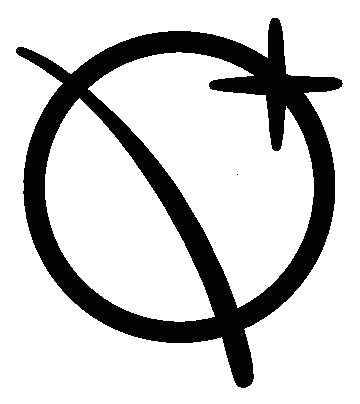
\includegraphics[height=75px]{LOGO.eps}
\end{minipage}%
\begin{minipage}{0.45\textwidth}
\begin{shaded*}
\begin{tabularx}{0.5\textwidth}{r|X}
\makecell[r]{\LARGE{\textbf{Young World}}\\ \LARGE{\textbf{Federalists}}} & \makecell[l]{\textbf{\href{https://www.ywf.world}{ywf.world}} \\ \textbf{\href{https://twitter.com/ywf_world}{@ywf\_world}}\\  
\textbf{\href{https://www.reddit.com/r/GlobalTribe/}{r/GlobalTribe}}}
\end{tabularx}
\end{shaded*}
\end{minipage}%
\begin{minipage}{0.3\textwidth}
\centering

\includegraphics[height=64px]{qrcode-discord.eps} 
\includegraphics[height=64px]{qrcode-facebook.eps}

\end{minipage}%


\end{document}
